%% Related Work
%%=========================================

\chapter{Related Work}
\label{ch:related_work}
This chapter presented related work that can lay the foundation for our system. Basing our system on the task of translation, we look closer at natural language processing, specifically recent work in the area of machine translation. Establishing the state of the art in this area, we present the underlying work that make up these systems by explaining their architecture and implementation.

%%=========================================

\section{Natural Language Processing}
\label{sec:natural_language_processing}
In 1954, a translation system developed at Georgetown University was demonstrated for the first time. The system did fully automatic translation of more than sixty sentences from Russian to English. One of the creators, Léon Dostert, predicted that automatic text-reading translations machines would be finished within three to five years \citep{hutchins1997first}. As research continued, the complexity of the linguistic problems became more and more apparent. Critics argued that the concept of fully automatic high quality translations that could produce translations indistinguishable from those of humans translators were impossible in principle \citep{hutchins2007machine}. National Science Foundation established the Automatic Language Processing Advisory Committee (ALPAC) in 1964, to carry out a study of the realities of machine translation. In 1966 they published their report that concluded that the use of machine translation was slower, less accurate and twice as expensive as human translation. The report also said that there was no immediate or predictable prospect of useful machine translation \citep{hutchins2007machine, national1966language, koehn2010statistical}. The ALPAC report led to a decrease of research in the area, but it did not stop completely.

It was first as the later half of the 1970s and the early 1980s that machine translation again saw a rise in popularity. The latter half of the 1980s also saw a general revival in interest in interlingua systems. This interest was motivated in part by artificial intelligence, which was also a research field that attracted much attention. Since the 1980s, new methods such as corpus-based approaches and statistical machine translation based systems. Speech translation has also seen growing interest since the late 1980s \citep{hutchins2007machine}.

\begin{figure}[H]
    \centering
    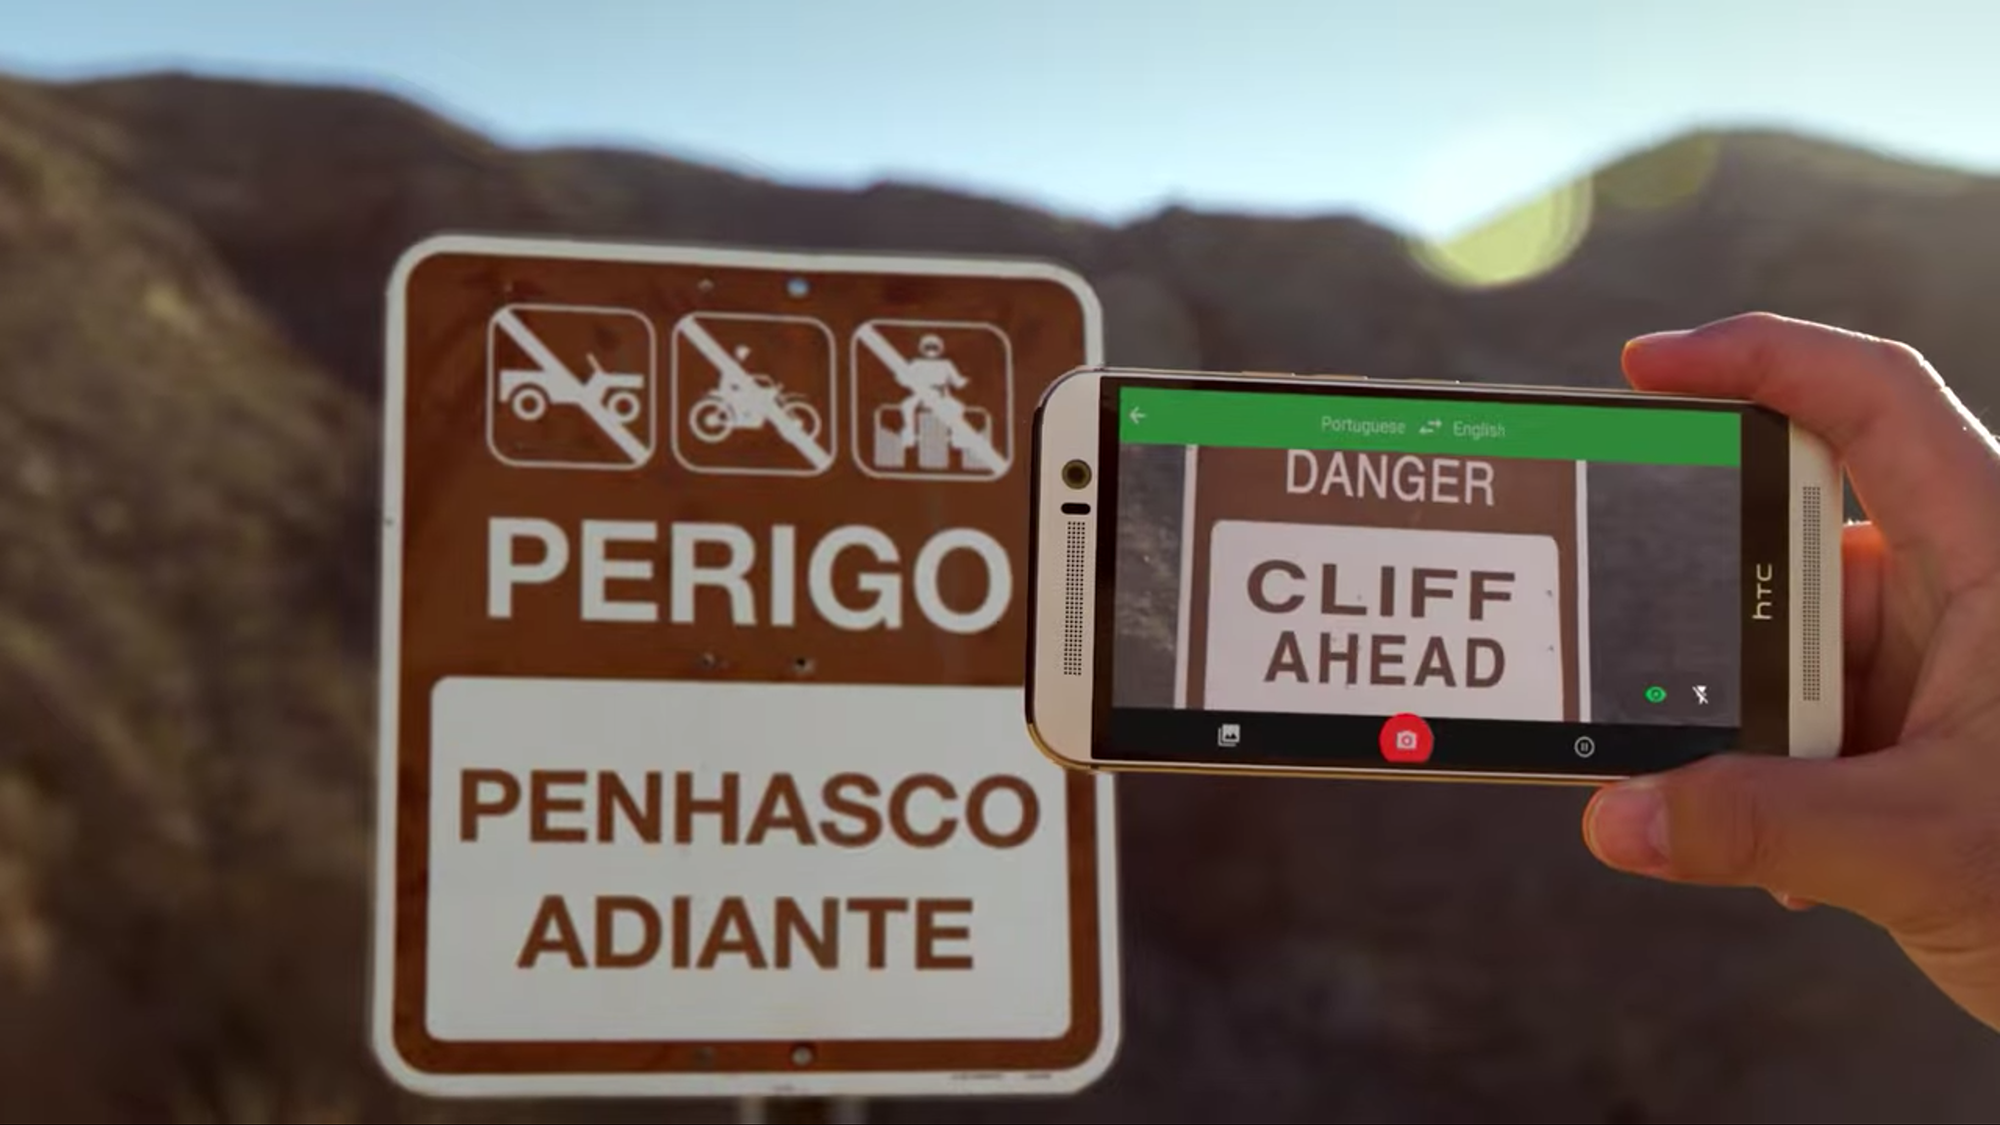
\includegraphics[width=0.7\textwidth]{fig/background_theory/google_translate_rt.png}
    \caption{The Google Translate app and its image translation feature}
    \label{fig:google-translate-rt}
\end{figure}

In recent years, online solution such as Google Translate\footnote{https://translate.google.com} and AltaVista's Babelfish\footnote{https://www.babelfish.com} has gained much popularity. Both services offers on-demand translation for free \citep{hutchins2007machine}. Google reported on their blog in 2016 that their service now supported over 100 languages, had more than 500 million users and translated more than 100 billion words a day \citep{turovsky2016googletranslate}. The native app for Google Translate has also become very popular. It offers the same functionality as their online counterpart, but also offer a few additional features, such as ``Word Lens" which translates images in place.

%%=========================================

\section{Statistical Machine Translation}
\begin{figure}[ht]
    \centering
    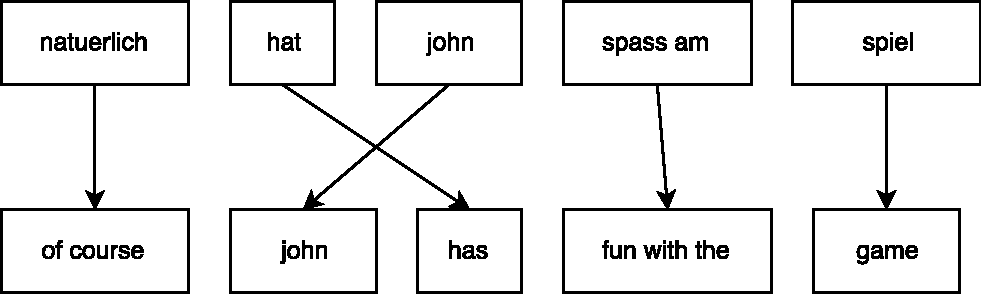
\includegraphics[width=0.7\textwidth]{fig/related_work/translation_de_en.pdf}
    \caption{Phrase-based translation of a German sentence to English}
    \label{fig:translation-phrase-based}
\end{figure}

For the past two decades or so, machine translation has taken a new direction. Instead of pre-defined rule-based systems, many modern machine translation systems attack the problem of machine translation with statistical methods and ideas from information theory \citep{brown1990statistical}. Statistical machine translation was born as an idea in the 1980s in the labs of IBM Research. The idea came in the wake of success of statistical methods in speech recognition. The idea was to model the translation task as a statistical optimization problem. Some of the best performing SMT systems today are phrase-based, an approach where the input sequence is broken up into a sequence of phrases, and these phrases are mapped one-to-one to output phrases, which may be reordered \citep{koehn2010statistical}. See Figure \ref{fig:translation-phrase-based} for illustration of a phrase-based translation of a German sentence to English.

Statistical machine translation has been the dominant translation paradigm for decades \citep{wu2016google}. Variants and implementations of SMT based systems have achieved state of the art performance in machine translation \citep{watanabe07onlinelargemargin}. There now also exists SMT systems on the commercial market, a market long dominated by the well-established rule-based methods \citep{hutchins2007machine}.

%%=========================================

\section{Neural Machine Translation}
Neural machine translation is another approach to machine translation that has emerged recently. This approach aims at building a jointly-tuned single neural network which is trained to maximize translation performance. This is a different approach from traditional statistical machine translation systems, where a translation system consists of sub components that are optimized separately \citep{wolk2015neural}. The great benefit of neural machine translation systems is its ability to learn directly, in an end-to-end fashion. 

In 2016, Google published their work on Google's Neural Machine Translation system, or GNMT for short. This system replaced their older statistical machine translation system that ran Google Translate \citep{turovsky2016googletranslatenmt}. GNMT uses the common sequence-to-sequence learning framework as proposed by \citep{sutskever2014sequence, wu2016google}. This framework uses multilayered Long Short-Term Memory (LSTM) to map the input sequence to a vector of a fixed dimensionality, and then another LSTM to decode the target sequence from the fixed vector. Their implementation is closely related to the work of \citep{kalchbrenner2013recurrent} who were the first to map the input sentence into a vector, and then back into a sentence. It also build heavily on the neural network architecture presented by \citep{cho2014learning}. They did this using LSTM-like RNN architecture, although their primary focus was to integrate their neural network into an SMT system \citep{cho2014learning, sutskever2014sequence}. The work of \citep{sutskever2014sequence} did the entire translation end-to-end and was not integrated with any other frameworks or systems. Their implementation achieved close-to-best results in an English to French translation task, and outperformed various SMT-based systems.

\begin{figure}[ht]
    \centering
    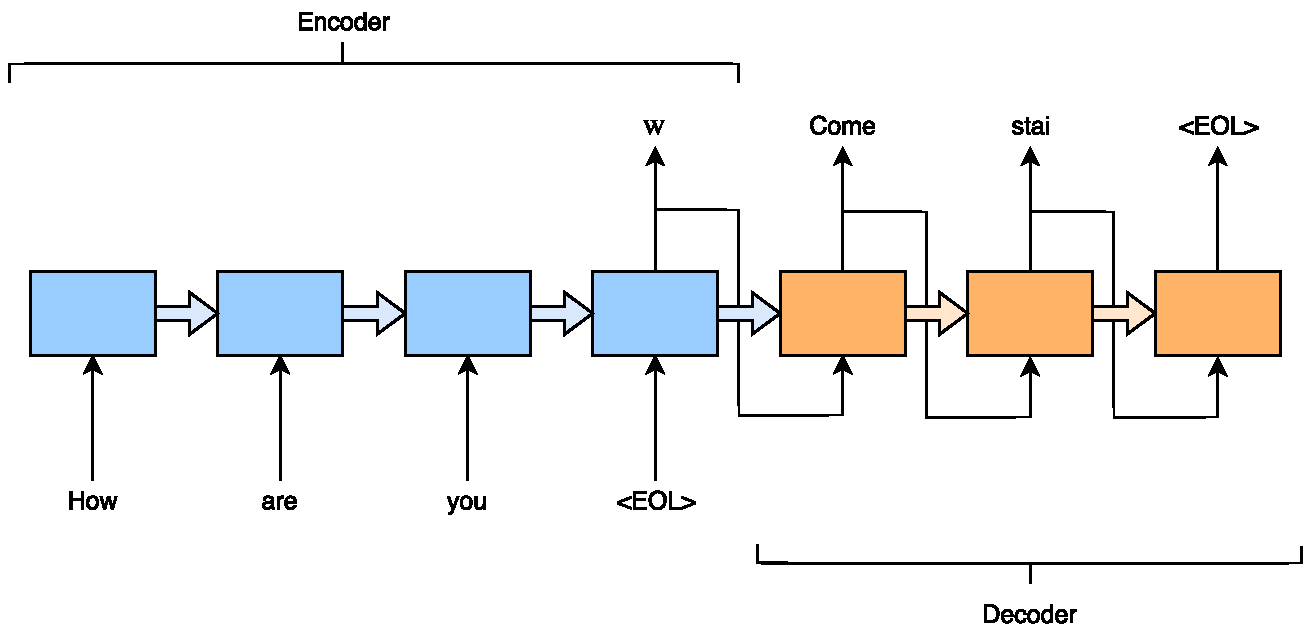
\includegraphics[width=0.8\textwidth]{fig/related_work/encoder_decoder_en_it.pdf}
    \caption{General translation approach in neural machine translation from an English sentence to Italian}
    \label{fig:machine-translation-encoder-decoder-simple}
\end{figure}

The encoder-decoder approach, as further explained in section \ref{sec:encoder-decoder}, has also been used as the foundation for various other NMT architectures. \citep{chung2016character} used the encoder-decoder general approach in their experiment, although they used bi-scale recurrent network with gated recurrent units (GRU), instead of LSTMs. They showed that their model, which did translation on a sequence of characters, without any explicit word segmentation, using a charachter-level decoder, could outperform the one with a subword-level decoder.

\citep{bahdanau2014neural} proposed another model, which did not use the fixed-length vector that the encoder produces. They argued that the fixed-length vector was a bottleneck in improving the performance of the encoder-decoder approach. Their argument was that the neural network needed to compress all the necessary information of a source sentence into a fixed-length vector, which may make make it difficult to cope with longer sentences. This was already shown in the analysis by \citep{cho2014properties}, where a variant of \citep{cho2014learning} as well as a novel network dubbed \textit{gated recursive convolutional neural network} were evaluated. Their evaluation showed that both architectures performed relatively well on short sentences, but suffered significantly as the length of the sentences increased. The model proposed by \citep{bahdanau2014neural} instead learns to align and translate joinly. It does this by encoding the input sequence into a sequence of vectors and chooses a subset of these vectors adaptively while decoding the translation. This model outperformed the basic encoder-decoder significantly in their experiments.

\iffalse
\begin{itemize}
    \item Talk fast about ``ORDER MATTERS: SEQUENCE TO SEQUENCE FOR SETS"
    \item Talk about ``Addressing the Rare Word Problem in Neural Machine Translation", this can be in greater detail
    \item At some point talk about something that also uses attention. Needs to present this too.
\end{itemize}
\fi

%%=========================================

\section{Encoder-Decoder}
\label{sec:encoder-decoder}
The encoder-decoder framework is centralized around two recurrent neural networks. The idea is to encode the input in the first neural network, and decode it in the second network. The first neural network, also called the encoder, reads the input sentence, a sequence of vectors \(X = (x_{1}, x_{2}, ..., x_{n})\). This sequence is then encoded into a vector \(c\), which may or may not be of fixed length.